\documentclass{article}
\usepackage{fullpage}
\usepackage[utf8]{inputenc}
\usepackage{pict2e}
\usepackage{amsmath}
\usepackage{enumitem}
\usepackage{eurosym}
\usepackage{mathtools}
\usepackage{amssymb, amsfonts, latexsym, cancel}
\setlength{\parskip}{0.3cm}
\usepackage{graphicx}
\usepackage{fontenc}
\usepackage{slashbox}
\usepackage{setspace}
\usepackage{gensymb}
\usepackage{accents}
\usepackage{adjustbox}
\setstretch{1.35}
\usepackage{bold-extra}
\usepackage{subcaption}
\usepackage{tcolorbox}
\usepackage{xcolor, colortbl}
\usepackage{wrapfig}
\usepackage{empheq}
\usepackage{array}
\usepackage{parskip}
\usepackage{arydshln}
\graphicspath{ {images/} }
\renewcommand*\contentsname{\color{black}Índice} 
\usepackage{array, multirow, multicol}
\definecolor{lightblue}{HTML}{007AFF}
\usepackage{color}
\usepackage{etoolbox}
\usepackage{listings}
\usepackage{mdframed}
\setlength{\parindent}{0pt}
\usepackage{underscore}
\usepackage{hyperref}
\usepackage{tikz}
\usepackage{tikz-cd}
\usetikzlibrary{shapes, positioning, patterns}
\usepackage{tikz-qtree}
\usepackage{biblatex}
\usepackage{pdfpages}
\usepackage{pgfplots}
\usepackage{pgfkeys}
\addbibresource{biblatex-examples.bib}
\usepackage[a4paper, left=1cm, right=1cm, top=1cm, bottom=1.5cm]{geometry}
\usepackage{titlesec}
\usepackage{titletoc}
\usepackage{tikz-3dplot}
\usepackage{kbordermatrix}
\usetikzlibrary{decorations.pathreplacing}
\newcommand{\Ej}{\textcolor{lightblue}{\underline{Ejemplo}}}
\setlength{\fboxrule}{1.5pt}

\newcommand{\bboxed}[1]{\fcolorbox{lightblue}{lightblue!10}{$#1$}}
\newcommand{\rboxed}[1]{\fcolorbox{red}{red!10}{$#1$}}

\DeclareMathOperator{\N}{\mathbb{N}}
\DeclareMathOperator{\Z}{\mathbb{Z}}
\DeclareMathOperator{\R}{\mathbb{R}}
\DeclareMathOperator{\Q}{\mathbb{Q}}
\DeclareMathOperator{\K}{\mathbb{K}}
\DeclareMathOperator{\im}{\imath}
\DeclareMathOperator{\jm}{\jmath}
\DeclareMathOperator{\col}{\mathrm{Col}}
\DeclareMathOperator{\fil}{\mathrm{Fil}}
\DeclareMathOperator{\rg}{\mathrm{rg}}
\DeclareMathOperator{\nuc}{\mathrm{nuc}}
\DeclareMathOperator{\dimf}{\mathrm{dimFil}}
\DeclareMathOperator{\dimc}{\mathrm{dimCol}}
\DeclareMathOperator{\dimn}{\mathrm{dimnuc}}
\DeclareMathOperator{\dimr}{\mathrm{dimrg}}
\DeclareMathOperator{\dom}{\mathrm{Dom}}
\DeclareMathOperator{\infi}{\int_{-\infty}^{+\infty}}
\newcommand{\dint}[2]{\int_{#1}^{#2}}

\newcommand{\bu}[1]{\textcolor{lightblue}{\underline{#1}}}
\newcommand{\lb}[1]{\textcolor{lightblue}{#1}}
\newcommand{\db}[1]{\textcolor{blue}{#1}}
\newcommand{\rc}[1]{\textcolor{red}{#1}}

\renewcommand{\CancelColor}{\color{lightblue}}
\newcommand{\code}[1]{\texttt{\textbf{#1}}}

\usepackage{textgreek}

\newcommand{\dx}{\:\mathrm{d}x}
\newcommand{\dt}{\:\mathrm{d}t}
\newcommand{\dy}{\:\mathrm{d}y}
\newcommand{\dz}{\:\mathrm{d}z}
\newcommand{\dth}{\:\mathrm{d}\theta}
\newcommand{\dr}{\:\mathrm{d}\rho}
\newcommand{\du}{\:\mathrm{d}u}
\newcommand{\dv}{\:\mathrm{d}v}
\newcommand{\tozero}[1]{\cancelto{0}{#1}}
\newcommand{\lbb}[2]{\textcolor{lightblue}{\underbracket[1pt]{\textcolor{black}{#1}}_{#2}}}
\newcommand{\dbb}[2]{\textcolor{blue}{\underbracket[1pt]{\textcolor{black}{#1}}_{#2}}}
\newcommand{\rub}[2]{\textcolor{red}{\underbracket[1pt]{\textcolor{black}{#1}}_{#2}}}

\titleformat{\section}{\normalfont\LARGE\bfseries}{\thesection.}{10 pt}{}

\title{\textbf{\huge Práctica 3 de Señales y Sistemas}\\ Señales y sistemas continuos en el dominio de la frecuencia}
\author{Francisco Javier Mercader Martínez\\ Rubén Gil Martínez}
\date{}

\usepackage{matlab-prettifier}

\lstset{
language=matlab,
basicstyle=\ttfamily\small,
keywordstyle=\color{blue},
commentstyle=\color{green!70!black},
stringstyle=\color{red},
showstringspaces=false,
breaklines=true,
frame=single,
backgroundcolor=\color{lightgray!10},
captionpos=b,
tabsize=2,
inputencoding=utf8,
literate={á}{{\'a}}1 {é}{{\'e}}1 {í}{{\'i}}1 {ó}{{\'o}}1 {ú}{{\'u}}1{ñ}{{\~n}}1
}

\everymath{\displaystyle}

\begin{document}
\maketitle

\section{Señales periódicas continuas. Series de Fourier}
Las ecuaciones que relacionan una señal periódica continua con su desarrollo en series de Fourier son \[ \begin{array}{l}
a_k=\dfrac{1}{T}\int_Tx(t)e^{-jk\frac{2\pi}{T}t}\dt\\
x(t)=\sum_{k=-\infty}^{+\infty}a_ke^{jk\frac{2\pi}{T}t}
\end{array} \]
En este ejercicio se implementarán las dos ecuaciones mediante funciones en MATLAB. Para ello es necesario simular la señal continua $x(t)$, discretizándola mediante un incremento de tiempo, $\Delta t$, dando lugar a la señal continua discretizada $x(k\Delta t)$.
\begin{enumerate}[leftmargin=*]
\item Genere en MATLAB las siguientes señales periódicas $(T=2)$, generando 3 periodos de cada una de ellas.

\begin{lstlisting}
% Definir el periodo y el paso de tiempo
T = 2; dt = 0.001;
% Crear el rango de tiempo para un periodo
t = -T/2:dt:T/2-dt;
\end{lstlisting}
\begin{enumerate}[label=\alph*)]
\item $x(t)=\begin{cases}
2, & 0<|t|<0.5\\
0,&0.5<|t|<1
\end{cases}$

\begin{lstlisting}
% a)
x = zeros(1, length(t));
ti = find(abs(t)<=0.5); x(ti) = 2;
ti = find(abs(t)> 0.5); x(ti) = 0;
figure(1), plot([t-T t t+T], [x x x], "LineWidth", 1.5, "color", "#007AFF");
xlabel('Tiempo (t)');
ylabel('x(t)');
title('$x(t)=\begin{cases}2 & 0<|t|<0.5\\0&0.5<|t|<1\end{cases}$','Interpreter','latex');
\end{lstlisting}

\begin{center}
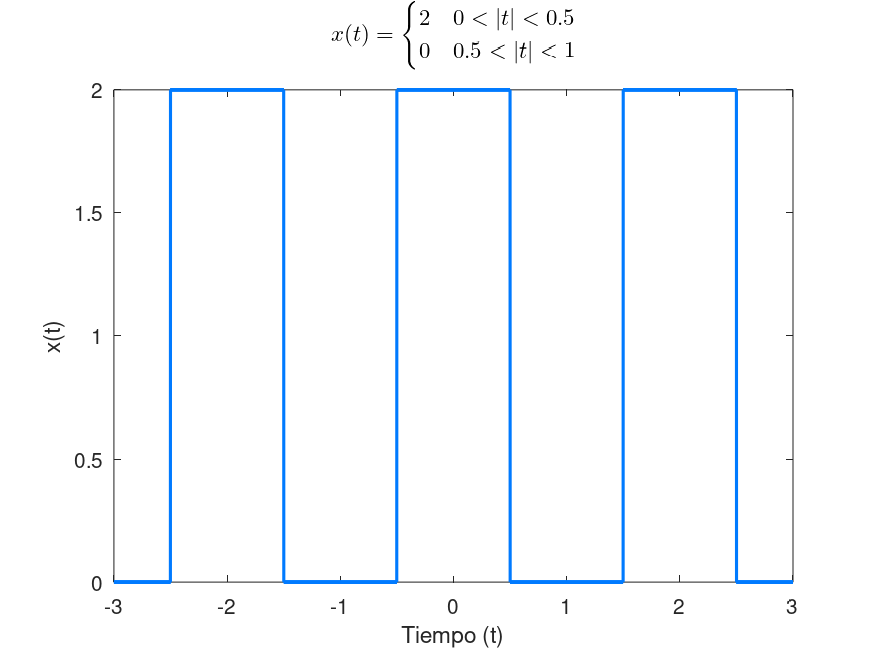
\includegraphics[width=0.5\linewidth]{Imágenes/Figura1}
\end{center}

\item $x(t)=0.8\sin(2\pi t)+0.6\cos(\pi t)-0.2\sin\left(3\pi t+\dfrac{\pi}{4}\right)$
\begin{lstlisting}
% b)
x = 0.8*sin(2*pi*t) + 0.6*cos(pi*t) - 0.2*sin(3*pi*t + pi/4);
figure(2), plot([t-T t t+T], [x x x], "LineWidth", 1.5, "color", "#007AFF");
xlabel('Tiempo (t)');
ylabel('x(t)');
title('$x(t)=0.8\sin(2\pi t)+0.6\cos(\pi t)-0.2\sin\left(3\pi t+\dfrac{\pi}{4}\right)$','Interpreter','latex');
\end{lstlisting}
\begin{center}
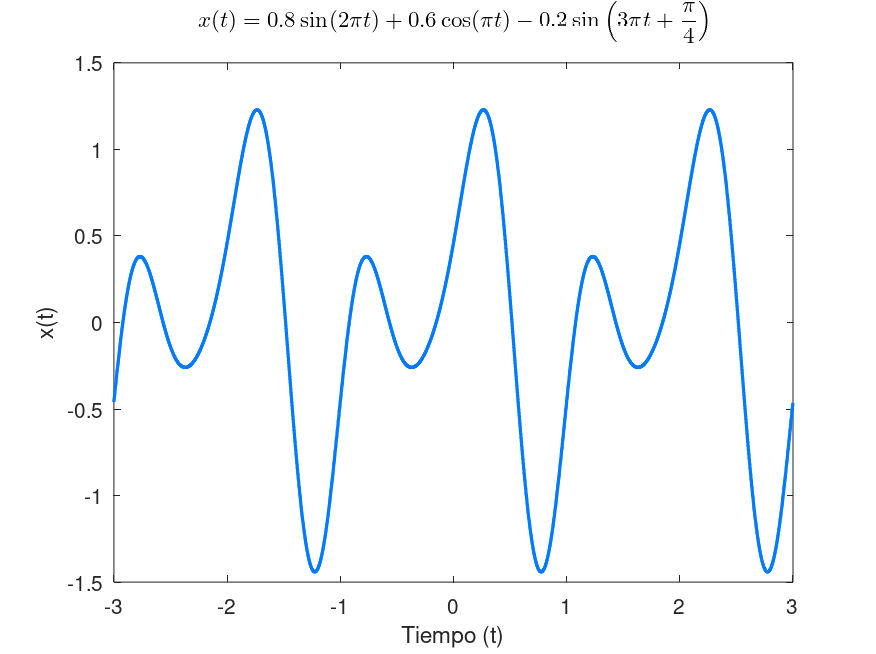
\includegraphics[width=0.5\linewidth]{Imágenes/Figura2}
\end{center}
\item $x(t)=\begin{cases}
2t, & 0<t<1\\
-2t,&-1\le t\le0
\end{cases}$
\begin{lstlisting}
% (c)
x = zeros(1, length(t));
ti = find(abs(t)>=-1 & abs(t)<0); x(ti) = -2*t(ti);
ti = find(abs(t)>0 & abs(t)<1); x(ti) = 2*t(ti);
figure(3), plot([t-T t t+T], [x x x], "LineWidth", 1.5, "color", "#007AFF");
xlabel('Tiempo (t)');
ylabel('x(t)');
title('$x(t)=\begin{cases}2t & 0<t<1\\-2t&-1\le t\le0\end{cases}$','Interpreter','latex');
\end{lstlisting}
\begin{center}
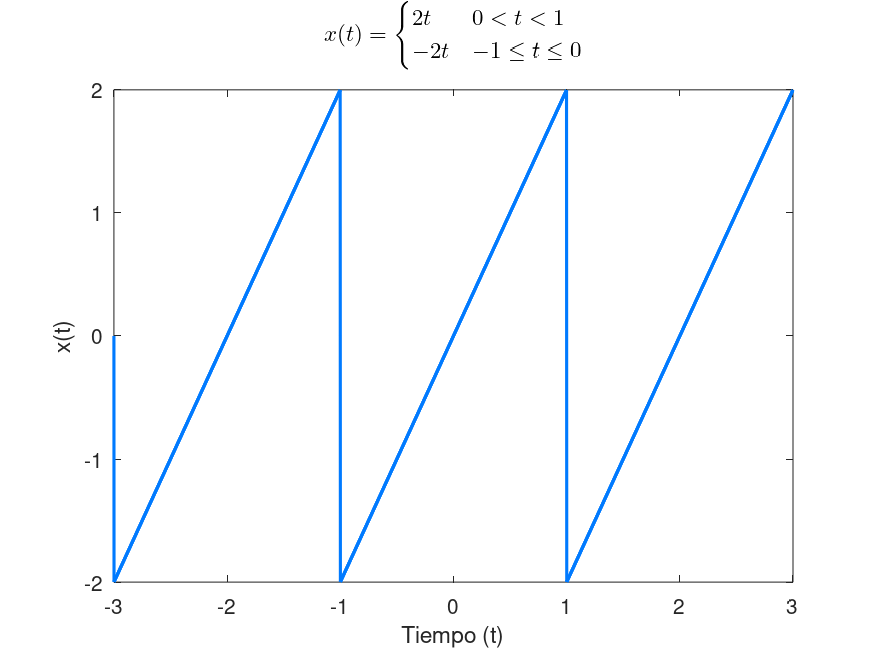
\includegraphics[width=0.5\linewidth]{Imágenes/Figura3}
\end{center}
\item $x(t)=0.5\delta(t),\:-1\le t<1$
\begin{lstlisting}
% (d)
ti = find(abs(t)==0); x(ti) = 0.5 * (1/dt);
figure(4), plot([t-T t t+T], [x x x], "LineWidth", 1.5, "color", "#007AFF");
xlabel('Tiempo (t)');
ylabel('x(t)');
title('$x(t)=0.5\delta(t),\,-1\le t<1$', 'Interpreter', 'latex')
\end{lstlisting}
\begin{center}
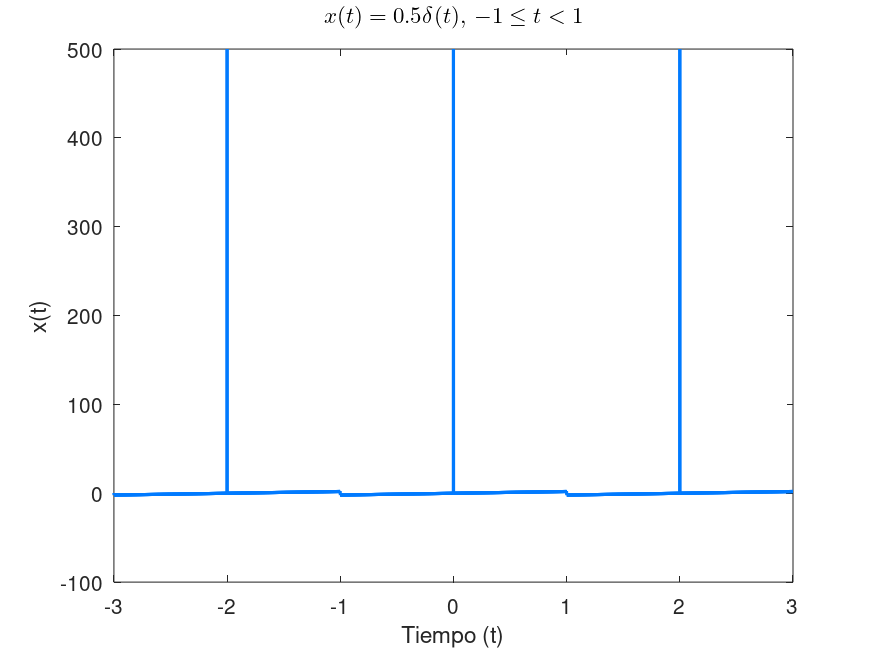
\includegraphics[width=0.5\linewidth]{Imágenes/Figura4}
\end{center}
\item $x(t)=\left|\sin\left(\dfrac{\pi}{2}t\right)\right|$
\begin{lstlisting}
% (e)
x = abs(sin(pi/2.*t));
figure(5), plot([t-T t t+T], [x x x], "LineWidth", 1.5, "color", "#007AFF");
xlabel('Tiempo (t)');
ylabel('x(t)');
title('$x(t)=\left|\sin\left(\dfrac{\pi}{2}t\right)\right|$', "Interpreter", "latex")
\end{lstlisting}
\begin{center}
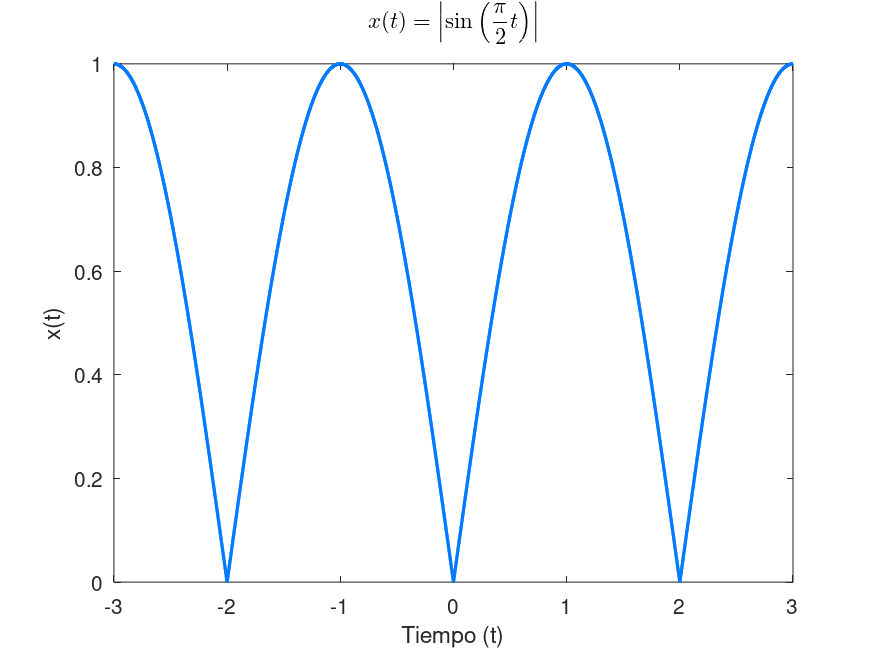
\includegraphics[width=0.5\linewidth]{Imágenes/Figura5}
\end{center}
\item $x(t)=e^{j2\pi t}+e^{-j3\pi t}$
\begin{lstlisting}
% (f)
x = exp(j*2*pi*t) + exp(-3*j*pi*t);
figure(6), plot([t-T t t+T], [x x x], "LineWidth", 1.5, "color", "#007AFF");
xlabel('Tiempo (t)');
ylabel('x(t)');
title('$x(t)=e^{j2\pi t}+e^{-j3\pi t}$', 'Interpreter', 'latex')
\end{lstlisting}
\begin{center}
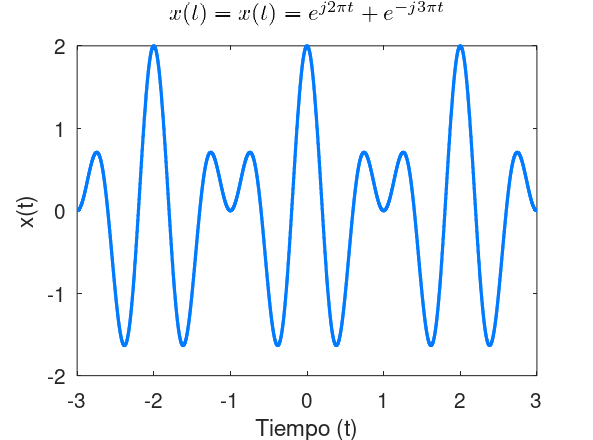
\includegraphics[width=0.5\linewidth]{Imágenes/Figura6}
\end{center}
\end{enumerate}

Ayuda: la señal (a) se obtiene mediante los comandos
\begin{lstlisting}
T = 2; dt = 0.001; t = -T/2:dt:T/2-dt;
x = zeros(1, length(t));
ti = find(abs(t)<=0.5); x(ti) = 2;
ti = find(abs(t)> 0.5); x(ti) = 0;
figure, plot([t-T t t+T], [x x x])
\end{lstlisting}
\item Repita el proceso para las señales a) c) y d), asumiendo un periodo T=4 y T=6. Razone los resultados obtenidos.

\pagebreak

\begin{lstlisting}
T = 4;dt = 0.001;
t = -T/2:dt:T/2-dt;
\end{lstlisting}

\begin{lstlisting}
% (a)
x = zeros(1, length(t));
ti = find(abs(t)<=0.5); x(ti) = 2;
ti = find(abs(t)> 0.5); x(ti) = 0;
figure(7), plot([t-T t t+T], [x x x], "LineWidth", 1.5, "color", "#007AFF");
xlabel('Tiempo (t)');
ylabel('x(t)');
title('$x(t)=\begin{cases}2 & 0<|t|<0.5\\0&0.5<|t|<1\end{cases}$','Interpreter','latex');

% (c)
x = zeros(1, length(t));
ti = find(abs(t)>=-1 & abs(t)<0); x(ti) = -2*t(ti);
ti = find(abs(t)>0 & abs(t)<1); x(ti) = 2*t(ti);
figure(8), plot([t-T t t+T], [x x x], "LineWidth", 1.5, "color", "#007AFF");
xlabel('Tiempo (t)');
ylabel('x(t)');
title('$x(t)=\begin{cases}2t & 0<t<1\\-2t&-1\le t\le0\end{cases}$','Interpreter','latex');

% (d)
x = zeros(1, length(t));
ti = find(abs(t)==0); x(ti) = 0.5 * (1/dt);
figure(9), plot([t-T t t+T], [x x x], "LineWidth", 1.5, "color", "#007AFF");
xlabel('Tiempo (t)');
ylabel('x(t)');
title('$x(t)=0.5\delta(t),\,-1\le t<1$', 'Interpreter', 'latex')
\end{lstlisting}
\begin{center}
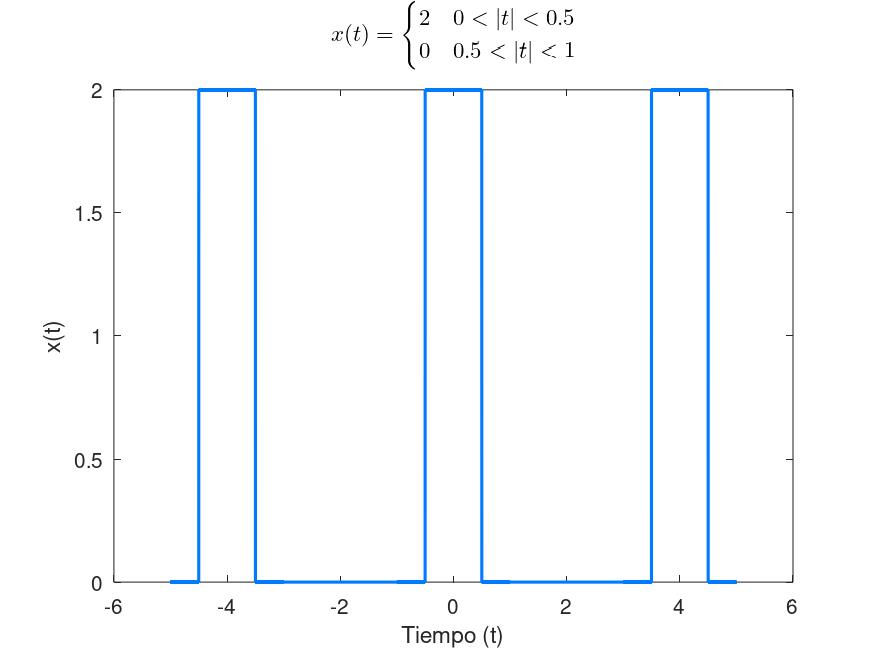
\includegraphics[width=0.4\linewidth]{Imágenes/Figura7}
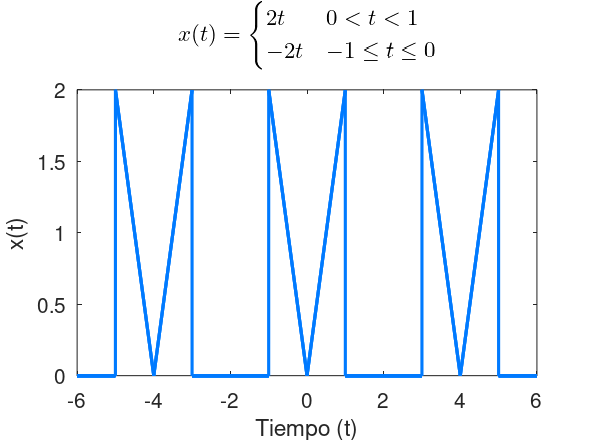
\includegraphics[width=0.4\linewidth]{Imágenes/Figura8}
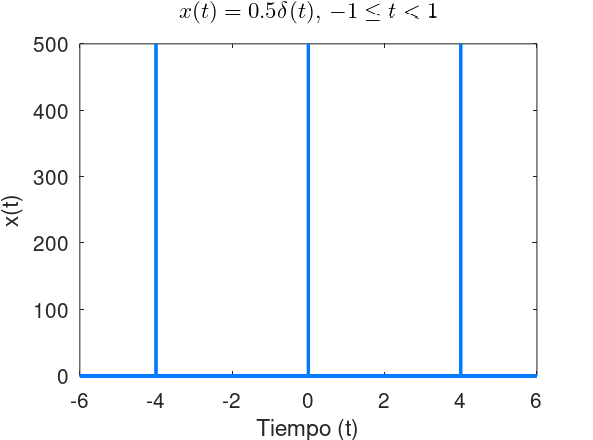
\includegraphics[width=0.4\linewidth]{Imágenes/Figura9}
\end{center}
\pagebreak
\begin{lstlisting}
T = 6; dt = 0.001;
t = -T/2:dt:T/2-dt;
\end{lstlisting}
\begin{lstlisting}
% (a)
x = zeros(1, length(t));
ti = find(abs(t)<=0.5); x(ti) = 2;
ti = find(abs(t)> 0.5); x(ti) = 0;
figure(10), plot([t-T t t+T], [x x x], "LineWidth", 1.5, "color", "#007AFF");
xlabel('Tiempo (t)');
ylabel('x(t)');
title('$x(t)=\begin{cases}2 & 0<|t|<0.5\\0&0.5<|t|<1\end{cases}$','Interpreter','latex');

% (c)
x = zeros(1, length(t));
ti = find(abs(t)>=-1 & abs(t)<0); x(ti) = -2*t(ti);
ti = find(abs(t)>0 & abs(t)<1); x(ti) = 2*t(ti);
figure(11), plot([t-T t t+T], [x x x], "LineWidth", 1.5, "color", "#007AFF");
xlabel('Tiempo (t)');
ylabel('x(t)');
title('$x(t)=\begin{cases}2t & 0<t<1\\-2t&-1\le t\le0\end{cases}$','Interpreter','latex');

% (d)
x = zeros(1, length(t));
ti = find(abs(t)==0); x(ti) = 0.5 * (1/dt);
figure(12), plot([t-T t t+T], [x x x], "LineWidth", 1.5, "color", "#007AFF");
xlabel('Tiempo (t)');
ylabel('x(t)');
title('$x(t)=0.5\delta(t),\,-1\le t<1$', 'Interpreter', 'latex')
\end{lstlisting}

\begin{center}
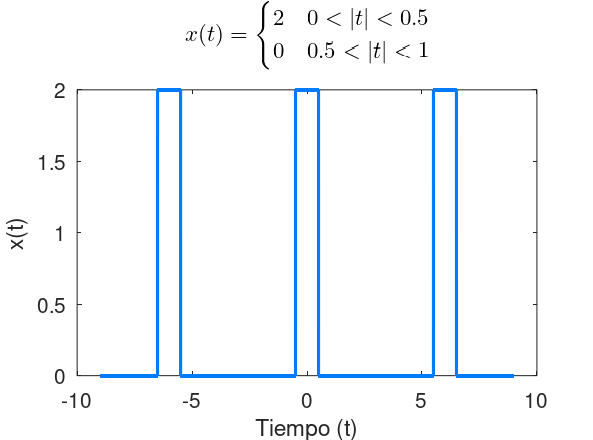
\includegraphics[width=0.4\linewidth]{Imágenes/Figura10}
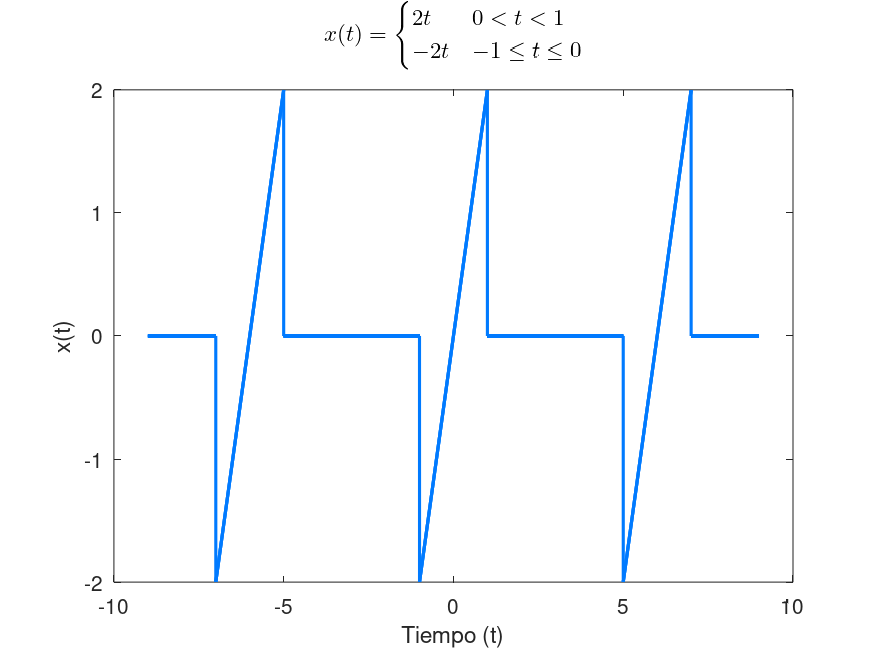
\includegraphics[width=0.4\linewidth]{Imágenes/Figura11}
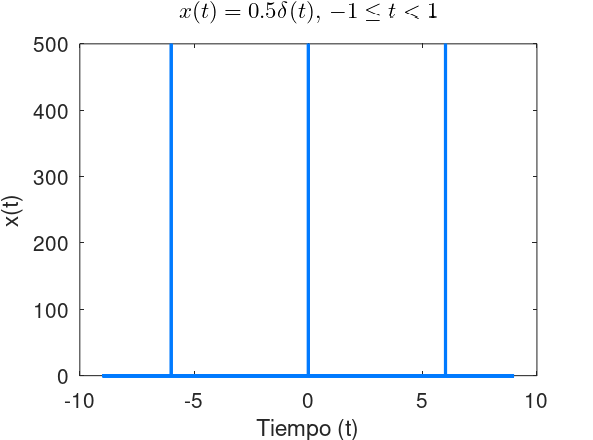
\includegraphics[width=0.4\linewidth]{Imágenes/Figura12}
\end{center}

Como se aumenta el periodo fundamental de las señales podemos observar que por la fórmula de su frecuencia angular $\left(\omega_0=\frac{2\pi}{T}\right)$ tenemos que se expande en el tiempo porque cuanto mayor sea el periodo fundamental, la señal tardará más tiempo en repetirse.

\item Cree la siguiente función de MATLAB que obtiene los coeficientes de la serie de Fourier (DSF) de una señal periódica:

\begin{lstlisting}
function ak = cfourier(x,T,N,dt)
t = -T/2:dt:T/2-dt;
ak = zeros(1,2*N+1);
for k = -N:N
    ak(k+N+1) = 1/T*sum(x.*exp(-j*k*2*pi/T*t))*dt;
end
\end{lstlisting}

donde \code{x} es una señal continua discretizada como las generadas anteriormente, \code{T} es el periodo de la señal, \code{N} es el orden del armónico más alto y \code{dt} es el paso temporal de discretación. El DSF queda almacenado en \code{ak} con el siguiente orden: \[ \left[a_{-N}a_{-N+1}a_{-N+2}\dots a_{-1}a_0a_1\dots a_{N-2}a_{N-1}a_{N}\right] \]
\item \textbf{Como estudio previo calcule analíticamente los desarrollos en series de Fourier de las señales del punto 1} y corrobore los resultados numéricos obtenidos con la función \code{cfourier}.

\begin{lstlisting}
% Definir el periodo y el paso de tiempo
T = 2; dt = 0.001; N=5;
t = -T/2:dt:T/2-dt;
\end{lstlisting}

\begin{lstlisting}
% (a)
x = zeros(1, length(t));
ti = find(abs(t)<=0.5); x(ti) = 2;
ti = find(abs(t)> 0.5); x(ti) = 0;
ak_a = cfourier(x, T, N, dt);
\end{lstlisting}
\begin{verbatim}
ak_a = 
   0.1273 + 0.0000i   0.0010 - 0.0000i  -0.2122 - 0.0000i  -0.0010 + 0.0000i   0.6366 - 0.0000i
   1.0010 +      0i   0.6366 + 0.0000i  -0.0010 - 0.0000i  -0.2122 + 0.0000i   0.0010 + 0.0000i
   0.1273 - 0.0000i
\end{verbatim}
\begin{lstlisting}
% (b)
x = 0.8*sin(2*pi*t) + 0.6*cos(pi*t) - 0.2*sin(3*pi*t + pi/4);
ak_b = cfourier(x, T, N, dt);
\end{lstlisting}

\begin{verbatim}
ak_b =
   0.0000 - 0.0000i  -0.0000 - 0.0000i  -0.0707 - 0.0707i  -0.0000 + 0.4000i   0.3000 + 0.0000i  
   -0.0000 +     0i   0.3000 - 0.0000i  -0.0000 - 0.4000i  -0.0707 + 0.0707i  -0.0000 + 0.0000i
   0.0000 + 0.0000i
\end{verbatim}

\begin{lstlisting}
% (c)
x = zeros(1, length(t));
ti = find(abs(t)>=-1 & abs(t)<0); x(ti) = -2*t(ti);
ti = find(abs(t)>0 & abs(t)<1); x(ti) = 2*t(ti);
ak_c = cfourier(x, T, N, dt);
\end{lstlisting}

\begin{verbatim}
ak_c =
   -0.0162 + 0.0000i   0.0000 + 0.0000i  -0.0450 + 0.0000i   0.0000 + 0.0000i  -0.4053 + 0.0000i
    1.0000 +      0i  -0.4053 - 0.0000i   0.0000 - 0.0000i  -0.0450 - 0.0000i   0.0000 - 0.0000i  
   -0.0162 - 0.0000i
\end{verbatim}

\begin{lstlisting}
% (d)
x = zeros(1, length(t));
ti = find(abs(t)==0); x(ti) = 0.5 * (1/dt);
ak_d = cfourier(x, T, N, dt);
\end{lstlisting}

\begin{verbatim}
ak_d =
   0.2500   0.2500   0.2500   0.2500   0.2500   0.2500   0.2500   0.2500   0.2500   0.2500   0.2500
\end{verbatim}

\begin{lstlisting}
% (e)
x = abs(sin(pi/2.*t));
ak_e = cfourier(x, T, N, dt);
\end{lstlisting}

\begin{verbatim}
ak_e =
  -0.0064 - 0.0000i  -0.0101 - 0.0000i  -0.0182 + 0.0000i  -0.0424 - 0.0000i  -0.2122 + 0.0000i   
   0.6366 +      0i  -0.2122 - 0.0000i  -0.0424 + 0.0000i  -0.0182 - 0.0000i  -0.0101 + 0.0000i  
  -0.0064 + 0.0000i
\end{verbatim}

\begin{lstlisting}
% (f)
x = exp(j*2*pi*t) + exp(-3*j*pi*t);
ak_f = cfourier(x, T, N, dt);
\end{lstlisting}

\begin{verbatim}
ak_f =
   -2.3575e-16 - 7.3283e-17i   3.4063e-16 + 5.8993e-17i   1.0000e+00 - 5.6710e-17i  
   -3.3348e-16 + 1.3077e-16i  -3.4729e-16 + 4.8116e-17i  -3.7292e-16 - 3.4807e-17i  
   -3.3980e-16 - 1.8739e-16i   1.0000e+00 + 5.8039e-17i   3.0022e-16 + 1.5665e-18i  
   -2.5388e-16 + 9.3413e-17i   3.3479e-17 + 5.4260e-17i
\end{verbatim}

\item Cree la siguiente función de MATLAB, que calcula la señal periódica a partir de su desarrollo en series de Fourier:

\begin{lstlisting}
function x = icfourier(ak,T,N,dt)
t = -T/2:dt:T/2-dt;
x = zeros(1,lenght(t));
for k = -N:N
    x = x + ak(k+N+1)*exp(j*k*2*pi/T*t);
end
\end{lstlisting}
\item Reconstruya a partir de los desarrollos mediante series de Fourier \code{ak} las señales a) c) d) y e) variando el máximo número de armónicos N en la reconstrucción. Comente los resultados obtenidos.

\begin{lstlisting}
% (a)
ic_a = icfourier(ak_a, T, N, dt);
% (c)
ic_c = icfourier(ak_c, T, N, dt);
% (d)
ic_d = icfourier(ak_d, T, N, dt);
% (e)
ic_e = icfourier(ak_e, T, N, dt);
\end{lstlisting}

A continuación van a aparecer dos variaciones de los valores obtenidos del apartado (a) utilizando \code{N=1} y \code{N=5}, en ese orden:

\begin{center}
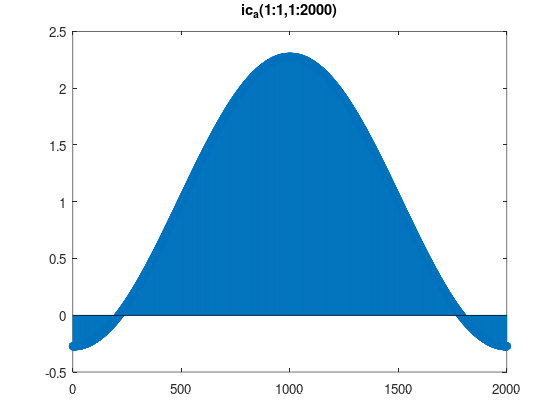
\includegraphics[width=0.45\linewidth]{Imágenes/prueba_n1}
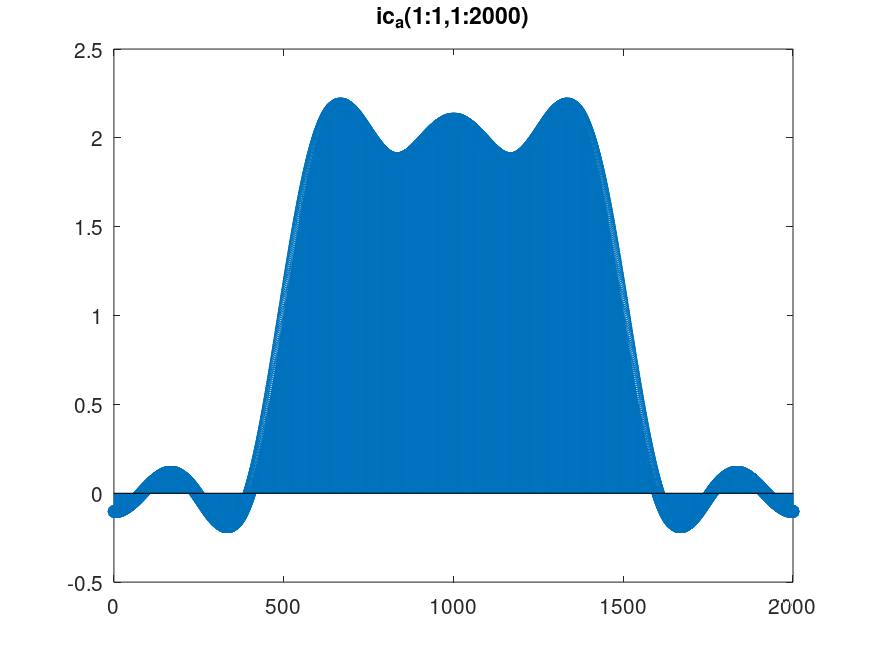
\includegraphics[width=0.45\linewidth]{Imágenes/prueba_n5}
\end{center}

Al aumentar el valor de \code{N} habrá más coeficientes y se obtendrá más información de la señal porque al reconstruirla usamos más coeficientes.

\item Verifique el cumplimiento del teorema de Parseval comparando los resultados \textbf{teóricos} y prácticos \[ \sum_{k=-\infty}^{\infty}|a_k|^2=\dfrac{1}{T}\int_{<T>}|x(t)|^2\dt \]

\begin{lstlisting}
% Calcular la suma de los cuadrados de los coeficientes de Fourier
sum_ak2_a = sum(abs(ak_a).^2); % sum_ak2_a = 1.9351
sum_ak2_b = sum(abs(ak_b).^2); % sum_ak2_b = 0.5200
sum_ak2_c = sum(abs(ak_c).^2); % sum_ak2_c = 1.3331
sum_ak2_d = sum(abs(ak_d).^2); % sum_ak2_d = 0.6875
sum_ak2_e = sum(abs(ak_e).^2); % sum_ak2_e = 0.4999
sum_ak2_f = sum(abs(ak_f).^2); % sum_ak2_f = 2.0000
\end{lstlisting}

\end{enumerate}
\section{Transformada de Fourier}
Las ecuaciones que relacionan una sñela con su transformada de Fourier son las siguientes: \[ X(\omega)=\int_{-\infty}^{\infty}x(t)e^{-j\omega t}\dt\qquad x(t)=\dfrac{1}{2\pi}\int_{-\infty}^{+\infty}X(\omega)e^{j\omega t}\mathrm{d}\omega \]
\subsection*{Cuestiones}
\begin{enumerate}[leftmargin=*]
\item Genere en MATLAB las siguientes señales aperiódicas, tomando un intervalo de discretación de 0.002, y considerando $-5\le t\le5$.
\begin{enumerate}[label=\alph*)]
\item $x(t)=\begin{cases}
1, & t\le0.6\\
0,&\text{resto}
\end{cases}$

\pagebreak

\begin{lstlisting}
% a)
t = -5:0.002:5;
x = zeros(size(t));
x(t <= 0.6) = 1;
figure(13); plot(t, x, "LineWidth", 1.5, "color", "#007AFF");
title(' $x(t)=\begin{cases}1, & t\le0.6\\0,&\text{resto}\end{cases}$', "Interpreter", "latex");
\end{lstlisting}
\begin{center}
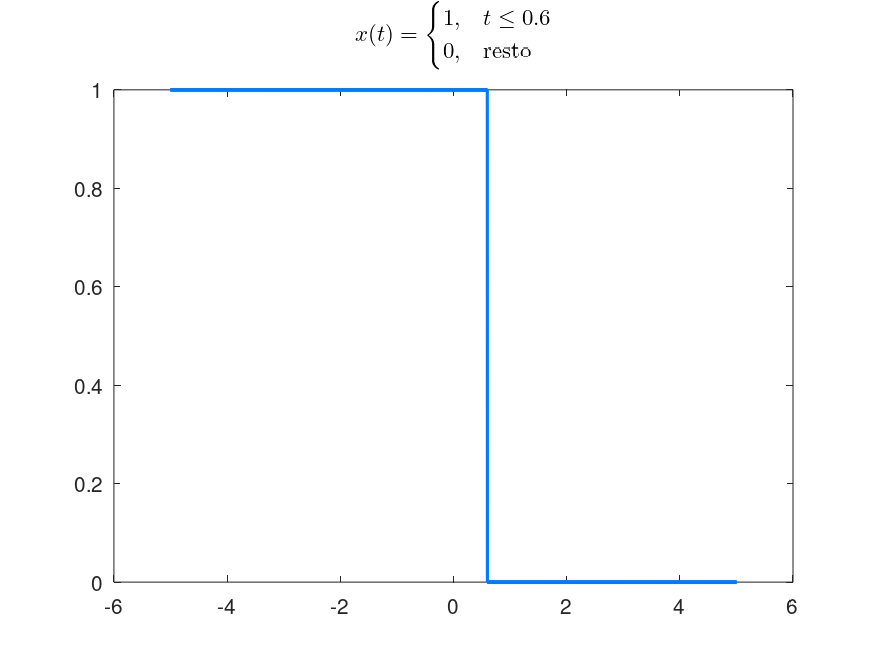
\includegraphics[width=0.5\linewidth]{Imágenes/Figura13}
\end{center}
\item $x(t)=\begin{cases}
1, & t\le0.2\\
0, & \mathrm{resto}
\end{cases}$
\begin{lstlisting}
% b)
t = -5:0.002:5;
x = zeros(size(t));
x(t <= 0.2) = 1;
figure(14); plot(t, x, "LineWidth", 1.5, "color", "#007AFF");
title('$x(t)=\begin{cases}1, & t\le0.2\\0, & \mathrm{resto}\end{cases}$', 'Interpreter', 'latex');
\end{lstlisting}
\begin{center}
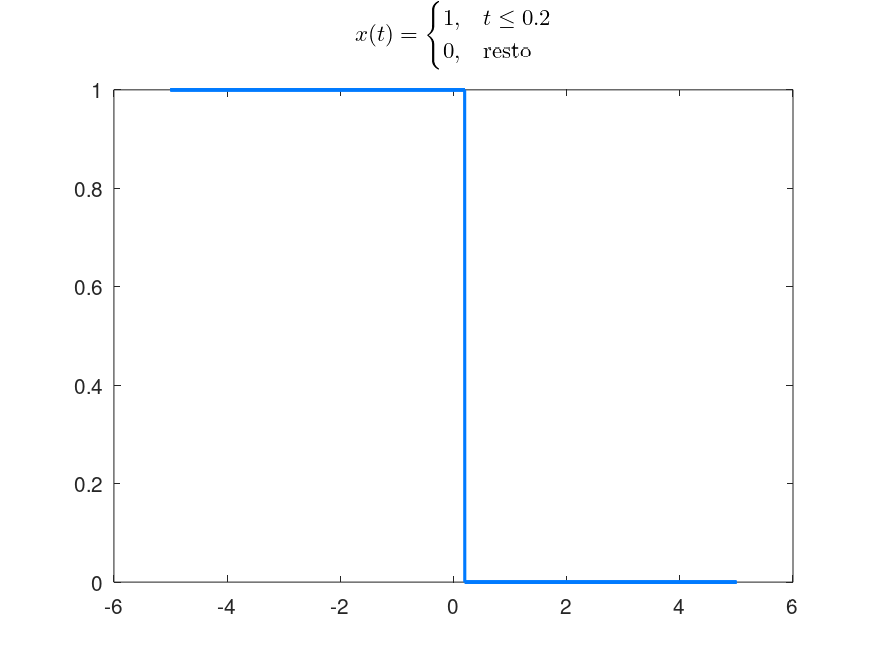
\includegraphics[width=0.5\linewidth]{Imágenes/Figura14}
\end{center}
\item $x(t)=\begin{cases}
0.5, & 0<t\le1\\
1-0.5t,&1<t\le2\\
0,& \mathrm{resto}
\end{cases}$

\pagebreak

\begin{lstlisting}
% c)
t = -5:0.002:5;
x = zeros(size(t));
x(0 < t & t <= 1) = 0.5;
x(1 < t & t <= 2) = 1 - 0.5 * t(1 < t & t <= 2);
figure(15); plot(t, x, "LineWidth", 1.5, "color", "#007AFF");
title('$x(t)=\begin{cases}0.5, & 0<t\le1\\1-0.5t,&1<t\le2\\0,& \mathrm{resto}\end{cases}$', "Interpreter", "latex");
\end{lstlisting}
\begin{center}
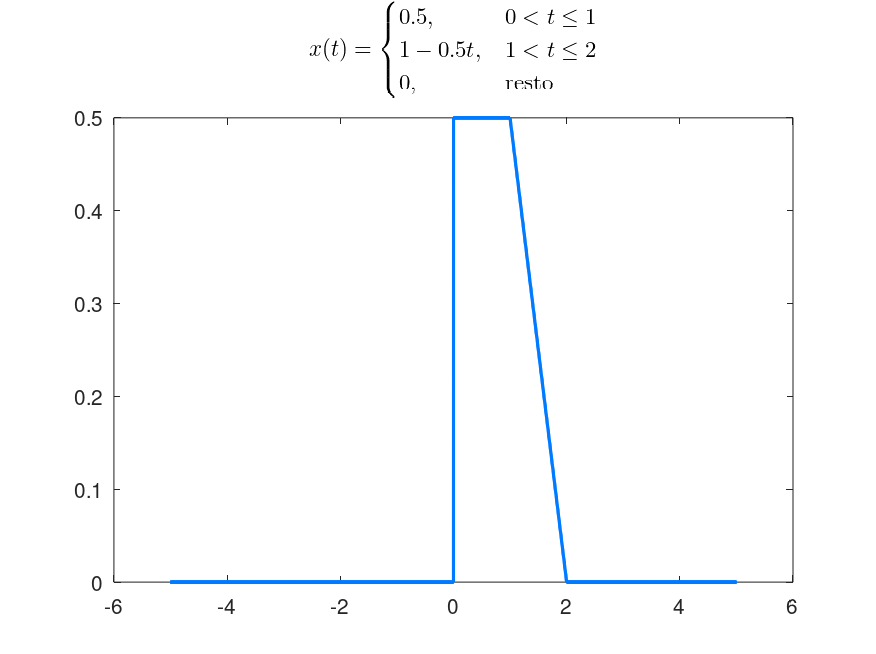
\includegraphics[width=0.5\linewidth]{Imágenes/Figura15}
\end{center}
\end{enumerate}
\item Suponiendo que las señales del punto 1 representaban el periodo de una señal periódica,
\begin{enumerate}[label=\roman*)]
\item Calcule su desarrollo en series de Fourier mediante \code{ak=cfourier(x,T,N,dt)}, y normalice por T (\code{ak=T*ak}). Al estar cada armónico está asociado a la frecuencia $k\dfrac{2\pi}{T}$, represente las series de Fourier normalizadas en el eje de frecuencias. Para ello emplee \code{stem(w,ak,'.')} y previamente defina el vector de frecuencias \code{w=2*\textpi*k/T}.
\begin{lstlisting}
% a)
x = zeros(size(t));
x(t <= 0.6) = 1;
T = length(x)*0.002;
N = 50;
dt = 0.002;
ak = cfourier(x, T, N, dt);
ak = T * ak;
k = 0:length(ak)-1;
w = 2*pi*k/T;
figure(16); stem(w, ak, '.', "LineWidth", 1.5, "color", "#007AFF", "MarkerSize", 10);
\end{lstlisting}
\begin{center}
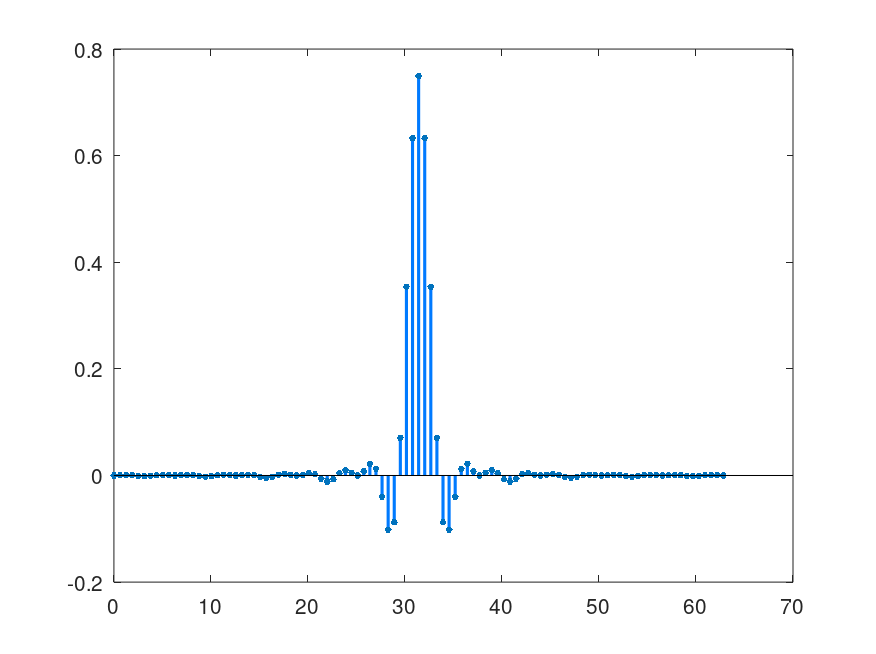
\includegraphics[width=0.5\linewidth]{Imágenes/Figura16}
\end{center}
\begin{lstlisting}
% b)
x = zeros(size(t));
x(t <= 0.2) = 1;
T = length(x)*0.002;
N = 50;
dt = 0.002;
ak = cfourier(x, T, N, dt);
ak = T * ak;
k = 0:length(ak)-1;
w = 2*pi*k/T;
figure(17); stem(w, ak, '.', "LineWidth", 1.5, "color", "#007AFF", "MarkerSize", 10);
\end{lstlisting}
\begin{center}
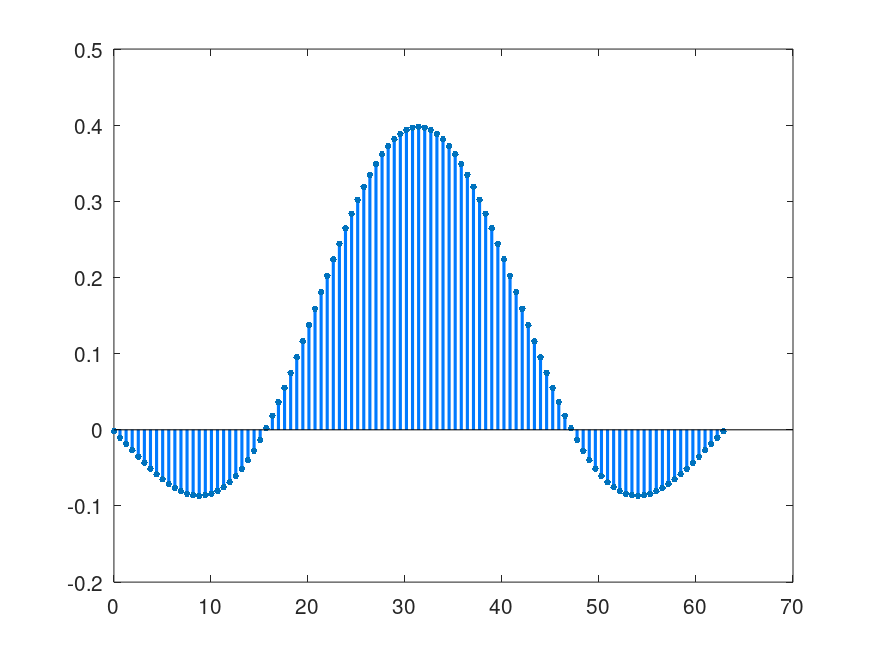
\includegraphics[width=0.5\linewidth]{Imágenes/Figura17}
\end{center}

\begin{lstlisting}
% c)
t = -5:0.002:5;
x = zeros(size(t));
x(0 < t & t <= 1) = 0.5;
x(1 < t & t <= 2) = 1 - 0.5 * t(1 < t & t <= 2);
T = length(x)*0.002;
N = 50;
dt = 0.002;
ak = cfourier(x, T, N, dt);
ak = T * ak;
k = 0:length(ak)-1;
w = 2*pi*k/T;
figure(18); stem(w, ak, '.', "LineWidth", 1.5, "color", "#007AFF", "MarkerSize", 10);
\end{lstlisting}
\begin{center}
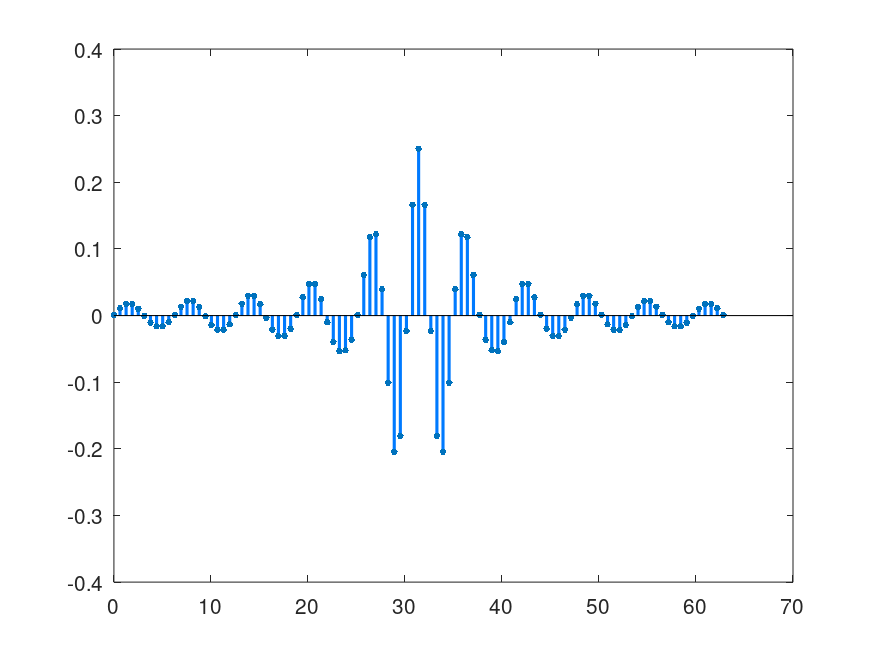
\includegraphics[width=0.5\linewidth]{Imágenes/Figura18}
\end{center}

\item Incremente la longitud del vector de la señal hacia ambos lados de la siguiente manera:
\begin{lstlisting}
Ti=floor(length(x)/2);
x=[zeros(1,Ti) x zeros(1,Ti)];
\end{lstlisting}

\begin{lstlisting}
% a)
x = zeros(size(t));
x(t <= 0.6) = 1;
Ti = floor(length(x)/2);
x = [zeros(1, Ti) x zeros(1, Ti)];
T = length(x)*dt;
N = 50;
dt = 0.002;
ak = cfourier(x, T, N, dt);
ak = T * ak;
k = 0:length(ak)-1;
w = 2*pi*k/T;
figure(19); stem(w, ak, '.', "LineWidth", 1.5, "color", "#007AFF", "MarkerSize", 10);
\end{lstlisting}
\begin{center}
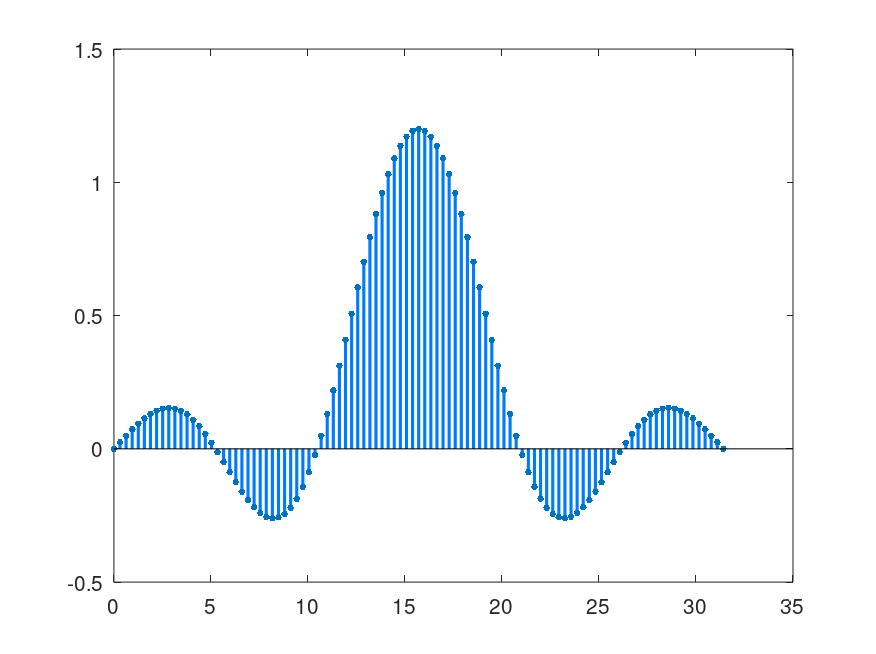
\includegraphics[width=0.5\linewidth]{Imágenes/Figura19}
\end{center}
\newpage
\begin{lstlisting}
% b)
x = zeros(size(t));
x(t <= 0.2) = 1;
Ti = floor(length(x)/2);
x = [zeros(1, Ti) x zeros(1, Ti)];
T = length(x)*dt;
N = 50;
dt = 0.002;
ak = cfourier(x, T, N, dt);
ak = T * ak;
k = 0:length(ak)-1;
w = 2*pi*k/T;
figure(20); stem(w, ak, '.', "LineWidth", 1.5, "color", "#007AFF", "MarkerSize", 10);
\end{lstlisting}
\begin{center}
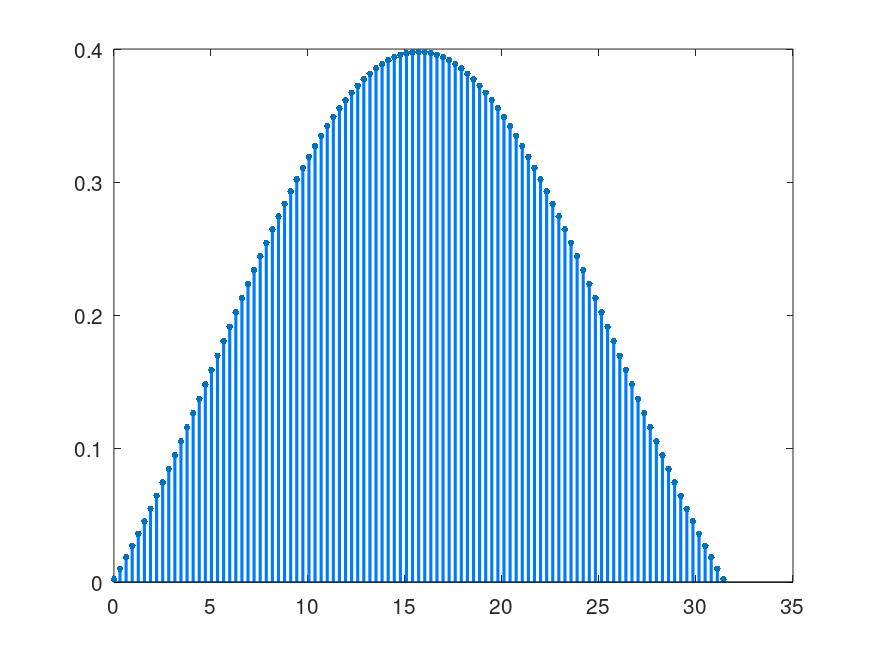
\includegraphics[width=0.5\linewidth]{Imágenes/Figura20}
\end{center}
\begin{lstlisting}
% c)
x = zeros(size(t));
x(0 < t & t <= 1) = 0.5;
x(1 < t & t <= 2) = 1 - 0.5 * t(1 < t & t <= 2);
Ti = floor(length(x)/2);
x = [zeros(1, Ti) x zeros(1, Ti)];
T = length(x)*dt;
N = 50;
dt = 0.002;
ak = cfourier(x, T, N, dt);
ak = T * ak;
k = 0:length(ak)-1;
w = 2*pi*k/T;
figure(21); stem(w, ak, '.', "LineWidth", 1.5, "color", "#007AFF", "MarkerSize", 10);
\end{lstlisting}
\begin{center}
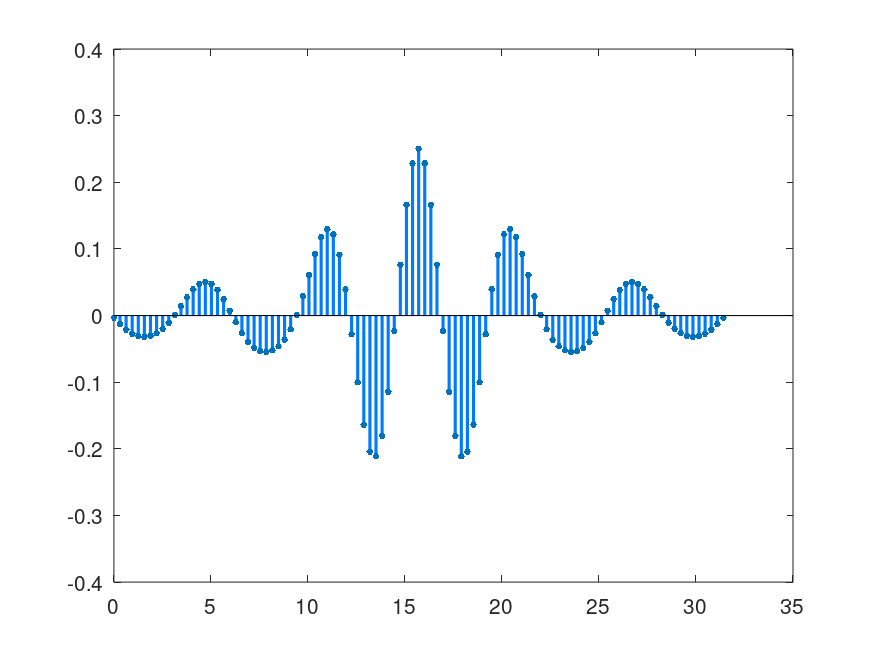
\includegraphics[width=0.5\linewidth]{Imágenes/Figura21}
\end{center}
\item Vuelva al paso \code{i} para obtener las nuevas series de Fourier normalizadas. Considere que:
\begin{itemize}[label=$-$]
\item El orden del máximo armónico a tener en cuenta es el doble que el previo (\code{N=2*N})
\item El nuevo periodo obtenido es el doble del previo (\code{T=2*T})
\end{itemize}
Repita este proceso (puede emplear un programa con un bucle \code{for}) y explique los resultados.

\begin{lstlisting}
% a)
T = 10;
t = -T/2:0.002:T/2-0.002;
x = zeros(size(t));
ti = find(abs(t) <= 0.6)
x(ti) = 1;
N = 50;
dt = 0.002;
% Bucle for para duplicar N y T
for i = 1:2
    Ti = floor(length(x)/2);
    x = [zeros(1, Ti) x zeros(1, Ti)];
    N = 2*N;
    T = 2*T;
    k = -N:N
    % Calcular ak y normalizar
    ak = cfourier(x, T, N, dt);
    ak = T * ak;

    % Definir k y w
    w = 2*pi*k/T;

    % Crear figura y representar las series de Fourier normalizadas
    figure; stem(w, ak, '.', "LineWidth", 1.5, "color", "#007AFF", "MarkerSize", 10);
end
\end{lstlisting}
\begin{center}
\includegraphics[width=0.45\linewidth]{"Imágenes/Figura22"}
\includegraphics[width=0.45\linewidth]{"Imágenes/Figura23"}
\end{center}
\begin{lstlisting}
% b)
T = 10;
t = -T/2:0.002:T/2-0.002;
x = zeros(size(t));
ti = find(abs(t) <= 0.2)
x(ti) = 1;
N = 50;
dt = 0.002;
% Bucle for para duplicar N y T
for i = 1:2
    Ti = floor(length(x)/2);
    x = [zeros(1, Ti) x zeros(1, Ti)];
    N = 2*N;
    T = 2*T;
    k = -N:N
    % Calcular ak y normalizar
    ak = cfourier(x, T, N, dt);
    ak = T * ak;
    % Definir k y w
    w = 2*pi*k/T;
    % Crear figura y representar las series de Fourier normalizadas
    figure; stem(w, ak, '.', "LineWidth", 1.5, "color", "#007AFF", "MarkerSize", 10);
end
\end{lstlisting}
\begin{center}
\includegraphics[width=0.45\linewidth]{"Imágenes/Figura24"}
\includegraphics[width=0.45\linewidth]{"Imágenes/Figura25"}
\end{center}
\newpage
\begin{lstlisting}
% b)
T = 10;
t = -T/2:0.002:T/2-0.002;
x = zeros(size(t));
ti = find(abs(t) <= 0.2)
x(ti) = 1;
N = 50;
dt = 0.002;
% Bucle for para duplicar N y T
for i = 1:2
    Ti = floor(length(x)/2);
    x = [zeros(1, Ti) x zeros(1, Ti)];
    N = 2*N;
    T = 2*T;
    k = -N:N
    % Calcular ak y normalizar
    ak = cfourier(x, T, N, dt);
    ak = T * ak;
    % Definir k y w
    w = 2*pi*k/T;
    % Crear figura y representar las series de Fourier normalizadas
    figure; stem(w, ak, '.', "LineWidth", 1.5, "color", "#007AFF", "MarkerSize", 10);
end
\end{lstlisting}
\begin{center}
\includegraphics[width=0.45\linewidth]{"Imágenes/Figura26"}
\includegraphics[width=0.45\linewidth]{"Imágenes/Figura27"}
\end{center}
\end{enumerate}
\item Implemente una función que obtenga la transformada de Fourier de una señal adaptando el programa de desarrollo en series de Fourier.
\begin{lstlisting}
function [X,w]=tfourier(x,t,dw,wmax)
\end{lstlisting}
\begin{itemize}[label=$-$]
\item El intervalo de frecuencias a calcular está entre \code{-wmax} y \code{wmax} (wmax\textless\textless\textpi/dt)
\item \code{dw} es la discretización en frecuencia en frecuencia
\item \code{w} es el vector con el eje frecuencia, su tamaño es el mismo que el de \code{x}.
\item \code{t} es el vector con el eje temporal, su tamaño es el mismo que el de \code{x}.
\end{itemize}
\pagebreak
\begin{lstlisting}
function [X,w] = tfourier(x,t,dw,wmax)
    % Crear el vector de frecuencias
    w = -wmax:dw:wmax;

    % Inicializar el vector de la Transformada de Fourier
    X = zeros(size(w));

    % Calcular la Transformada de Fourier para cada frecuencia
    for k = 1:length(w)
        X(k) = sum(x .* exp(-1i * w(k) * t));
    end
end
\end{lstlisting}
\item Empleando en la propiedad de la dualidad de la transformada de Fourier implemente una función que calcule la transformada inversa de Fourier haciendo uso de la función de la transformada directa.
\begin{lstlisting}
function [X,w]=itfourier(x,t,dw,wmax)
\end{lstlisting}


\begin{lstlisting}
function [X,t] = itfourier(x,w,dw,tmax)
    % Aplicar la Transformada de Fourier a la señal en el dominio de la frecuencia
    [x_tilde, t] = tfourier(x,w,dw,tmax);

    % Escalar la señal y tomar la parte real para obtener la señal en el dominio del tiempo
    X = real(dw/(2*pi) * x_tilde);
end
\end{lstlisting}

\item Verifique el correcto cumplimiento de las siguientes propiedades de la transformada de Fourier emplenado la función \code{tfourier}:
\begin{enumerate}[label=\roman*)]
\item Propiedad de linealidad $X(\omega)+Y(\omega)\longleftrightarrow x(t)+y(t)$ (emplee las señales a y b).
\item Desplazamiento en el tiempo $e^{-j\omega t_0}X(\omega)\longleftrightarrow x(t-t_0)$ (emplee señal b).
\item Inversión $X(-\omega)\longleftrightarrow x(-t)$ (emplee señal c).
\item Conjugación $X(\omega)^*\longleftrightarrow x(-t)^*$ (emplee señal c).
\item $\mathrm{Real}\{X(\omega)\}\longleftrightarrow\text{ Parte real}\{x(t)\}$ (emplee señal c).
\item $\mathrm{Imag}\{X(\omega)\}\longleftrightarrow\text{ Parte impar}\{x(t)\}$ (emplee señal c).
\end{enumerate}
\end{enumerate}
\end{document}